% faultsim module-level architecture diagram.
%
% Compile standalone:
%   pdflatex architecture.tex
%
% Or include in a paper:
%   % faultsim module-level architecture diagram.
%
% Compile standalone:
%   pdflatex architecture.tex
%
% Or include in a paper:
%   % faultsim module-level architecture diagram.
%
% Compile standalone:
%   pdflatex architecture.tex
%
% Or include in a paper:
%   % faultsim module-level architecture diagram.
%
% Compile standalone:
%   pdflatex architecture.tex
%
% Or include in a paper:
%   \input{figures/architecture}                 % just the tikzpicture
%   (wrap it in \begin{figure} ... \end{figure} in the host document)
%
% Required packages (already loaded below for standalone use):
%   tikz, with libraries: positioning, arrows.meta, shapes.geometric, calc

\documentclass[tikz,border=8pt]{standalone}
\usepackage{tikz}
\usetikzlibrary{positioning, arrows.meta, shapes.geometric, calc}

\begin{document}
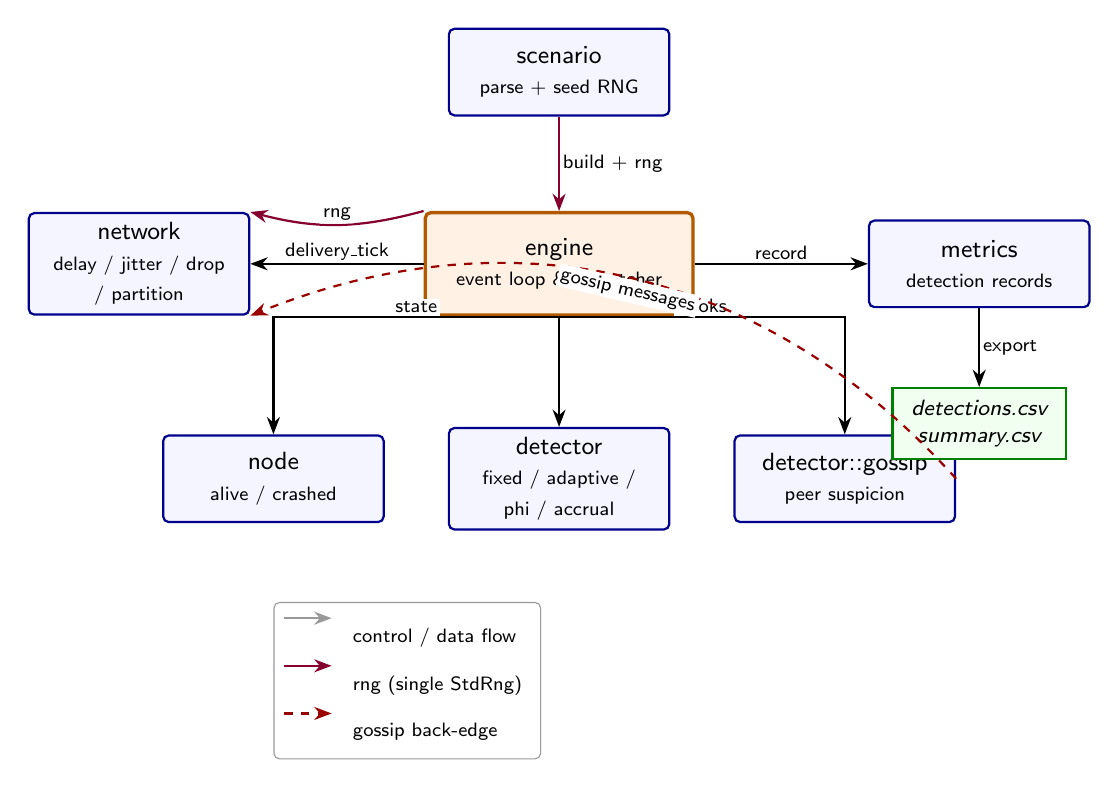
\begin{tikzpicture}[
    font=\sffamily\small,
    node distance=14mm and 18mm,
    every node/.style={align=center},
    %% module box: a service that the Engine calls into
    module/.style={
        draw, rounded corners=2pt, thick,
        minimum width=28mm, minimum height=11mm,
        fill=blue!4, draw=blue!55!black
    },
    %% the central event-loop module
    core/.style={
        draw, rounded corners=2pt, very thick,
        minimum width=34mm, minimum height=13mm,
        fill=orange!10, draw=orange!70!black
    },
    %% terminal artifact (CSV output)
    artifact/.style={
        draw, thick,
        minimum width=22mm, minimum height=9mm,
        fill=green!6, draw=green!50!black,
        font=\sffamily\footnotesize\itshape
    },
    %% data/control flow
    flow/.style={-{Stealth[length=2.2mm]}, thick},
    %% special-case gossip back-edge
    gossip/.style={-{Stealth[length=2.2mm]}, thick, dashed, draw=red!60!black},
    %% rng flow
    rng/.style={-{Stealth[length=2.2mm]}, thick, draw=purple!70!black},
    %% edge label
    elab/.style={font=\sffamily\scriptsize, fill=white, inner sep=1pt}
]

%%-------------------------------------------------------------- nodes
\node[module]                              (scenario)   {scenario\\\scriptsize parse + seed RNG};

\node[core,    below=12mm of scenario]     (engine)     {engine\\\scriptsize event loop \& dispatcher};

\node[module,  left=22mm of engine]        (network)    {network\\\scriptsize delay / jitter / drop\\\scriptsize / partition};

\node[module,  right=22mm of engine]       (metrics)    {metrics\\\scriptsize detection records};

\node[module,  below=14mm of engine]       (detector)   {detector\\\scriptsize fixed / adaptive /\\\scriptsize phi / accrual};

\node[module,  left=8mm of detector]       (node)       {node\\\scriptsize alive / crashed};

\node[module,  right=8mm of detector]      (gossip)     {detector::gossip\\\scriptsize peer suspicion};

\node[artifact, below=10mm of metrics]     (csv)        {detections.csv\\summary.csv};

%%-------------------------------------------------------------- edges
% scenario builds engine; rng enters here
\draw[rng] (scenario) -- node[elab,right] {build + rng} (engine);

% engine queries network for delivery_tick
\draw[flow] (engine.west) -- node[elab,above] {delivery\_tick} (network.east);

% engine writes to metrics
\draw[flow] (engine.east) -- node[elab,above] {record} (metrics.west);

% engine dispatches to nodes (state mutation) and detectors (hooks)
\draw[flow] (engine.south) -| node[elab,pos=0.25,above] {state} (node.north);
\draw[flow] (engine.south) --                                (detector.north);
\draw[flow] (engine.south) -| node[elab,pos=0.25,above] {hooks} (gossip.north);

% rng also flows from engine to network on every delivery_tick call
\draw[rng] (engine.north west) to[bend left=15] node[elab,above,sloped] {rng}  (network.north east);

% gossip is the one detector that produces messages back through the network
\draw[gossip] (gossip.east) to[bend right=35]
    node[elab,sloped,below] {gossip messages}
    (network.south east);

% metrics writes the CSV artifacts
\draw[flow] (metrics) -- node[elab,right] {export} (csv);

%%-------------------------------------------------------------- legend
\matrix [draw=black!40, rounded corners=2pt, fill=white,
         row sep=1pt, column sep=4pt,
         font=\sffamily\scriptsize,
         below=10mm of node, anchor=north west] (legend) {
  \draw[flow]   (0,0) -- (6mm,0); & \node {control / data flow}; \\
  \draw[rng]    (0,0) -- (6mm,0); & \node {rng (single StdRng)};  \\
  \draw[gossip] (0,0) -- (6mm,0); & \node {gossip back-edge};     \\
};

\end{tikzpicture}
\end{document}
                 % just the tikzpicture
%   (wrap it in \begin{figure} ... \end{figure} in the host document)
%
% Required packages (already loaded below for standalone use):
%   tikz, with libraries: positioning, arrows.meta, shapes.geometric, calc

\documentclass[tikz,border=8pt]{standalone}
\usepackage{tikz}
\usetikzlibrary{positioning, arrows.meta, shapes.geometric, calc}

\begin{document}
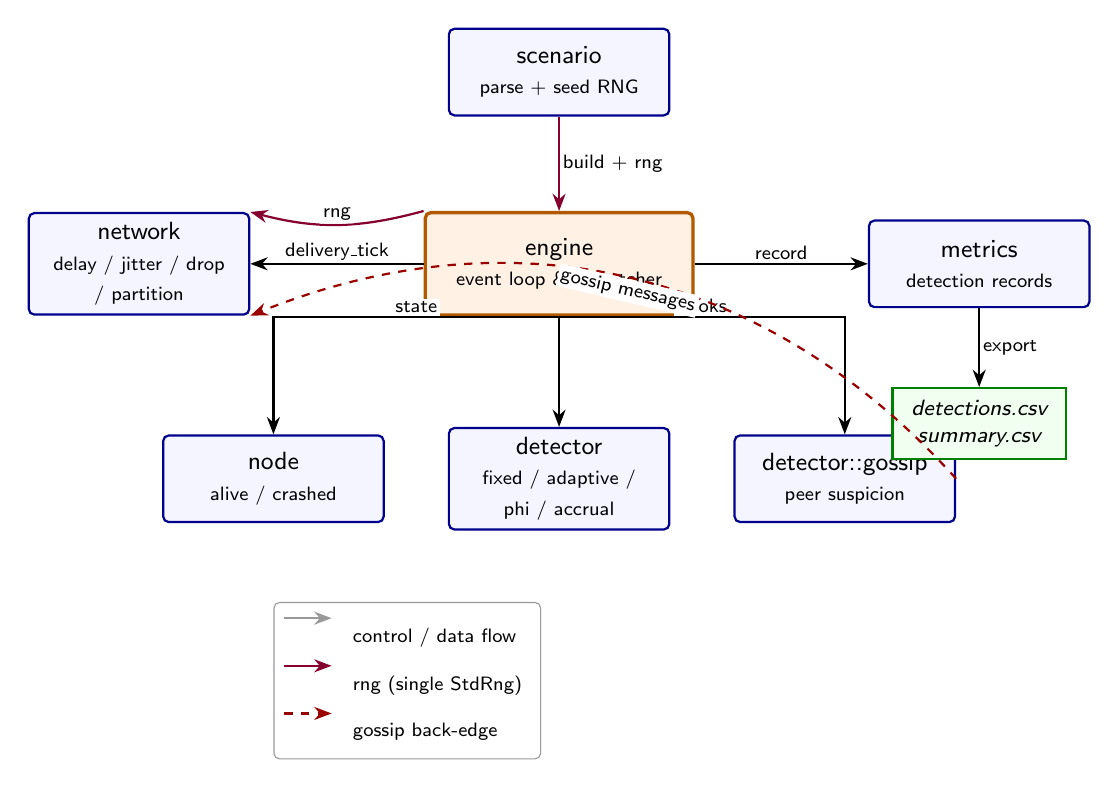
\begin{tikzpicture}[
    font=\sffamily\small,
    node distance=14mm and 18mm,
    every node/.style={align=center},
    %% module box: a service that the Engine calls into
    module/.style={
        draw, rounded corners=2pt, thick,
        minimum width=28mm, minimum height=11mm,
        fill=blue!4, draw=blue!55!black
    },
    %% the central event-loop module
    core/.style={
        draw, rounded corners=2pt, very thick,
        minimum width=34mm, minimum height=13mm,
        fill=orange!10, draw=orange!70!black
    },
    %% terminal artifact (CSV output)
    artifact/.style={
        draw, thick,
        minimum width=22mm, minimum height=9mm,
        fill=green!6, draw=green!50!black,
        font=\sffamily\footnotesize\itshape
    },
    %% data/control flow
    flow/.style={-{Stealth[length=2.2mm]}, thick},
    %% special-case gossip back-edge
    gossip/.style={-{Stealth[length=2.2mm]}, thick, dashed, draw=red!60!black},
    %% rng flow
    rng/.style={-{Stealth[length=2.2mm]}, thick, draw=purple!70!black},
    %% edge label
    elab/.style={font=\sffamily\scriptsize, fill=white, inner sep=1pt}
]

%%-------------------------------------------------------------- nodes
\node[module]                              (scenario)   {scenario\\\scriptsize parse + seed RNG};

\node[core,    below=12mm of scenario]     (engine)     {engine\\\scriptsize event loop \& dispatcher};

\node[module,  left=22mm of engine]        (network)    {network\\\scriptsize delay / jitter / drop\\\scriptsize / partition};

\node[module,  right=22mm of engine]       (metrics)    {metrics\\\scriptsize detection records};

\node[module,  below=14mm of engine]       (detector)   {detector\\\scriptsize fixed / adaptive /\\\scriptsize phi / accrual};

\node[module,  left=8mm of detector]       (node)       {node\\\scriptsize alive / crashed};

\node[module,  right=8mm of detector]      (gossip)     {detector::gossip\\\scriptsize peer suspicion};

\node[artifact, below=10mm of metrics]     (csv)        {detections.csv\\summary.csv};

%%-------------------------------------------------------------- edges
% scenario builds engine; rng enters here
\draw[rng] (scenario) -- node[elab,right] {build + rng} (engine);

% engine queries network for delivery_tick
\draw[flow] (engine.west) -- node[elab,above] {delivery\_tick} (network.east);

% engine writes to metrics
\draw[flow] (engine.east) -- node[elab,above] {record} (metrics.west);

% engine dispatches to nodes (state mutation) and detectors (hooks)
\draw[flow] (engine.south) -| node[elab,pos=0.25,above] {state} (node.north);
\draw[flow] (engine.south) --                                (detector.north);
\draw[flow] (engine.south) -| node[elab,pos=0.25,above] {hooks} (gossip.north);

% rng also flows from engine to network on every delivery_tick call
\draw[rng] (engine.north west) to[bend left=15] node[elab,above,sloped] {rng}  (network.north east);

% gossip is the one detector that produces messages back through the network
\draw[gossip] (gossip.east) to[bend right=35]
    node[elab,sloped,below] {gossip messages}
    (network.south east);

% metrics writes the CSV artifacts
\draw[flow] (metrics) -- node[elab,right] {export} (csv);

%%-------------------------------------------------------------- legend
\matrix [draw=black!40, rounded corners=2pt, fill=white,
         row sep=1pt, column sep=4pt,
         font=\sffamily\scriptsize,
         below=10mm of node, anchor=north west] (legend) {
  \draw[flow]   (0,0) -- (6mm,0); & \node {control / data flow}; \\
  \draw[rng]    (0,0) -- (6mm,0); & \node {rng (single StdRng)};  \\
  \draw[gossip] (0,0) -- (6mm,0); & \node {gossip back-edge};     \\
};

\end{tikzpicture}
\end{document}
                 % just the tikzpicture
%   (wrap it in \begin{figure} ... \end{figure} in the host document)
%
% Required packages (already loaded below for standalone use):
%   tikz, with libraries: positioning, arrows.meta, shapes.geometric, calc

\documentclass[tikz,border=8pt]{standalone}
\usepackage{tikz}
\usetikzlibrary{positioning, arrows.meta, shapes.geometric, calc}

\begin{document}
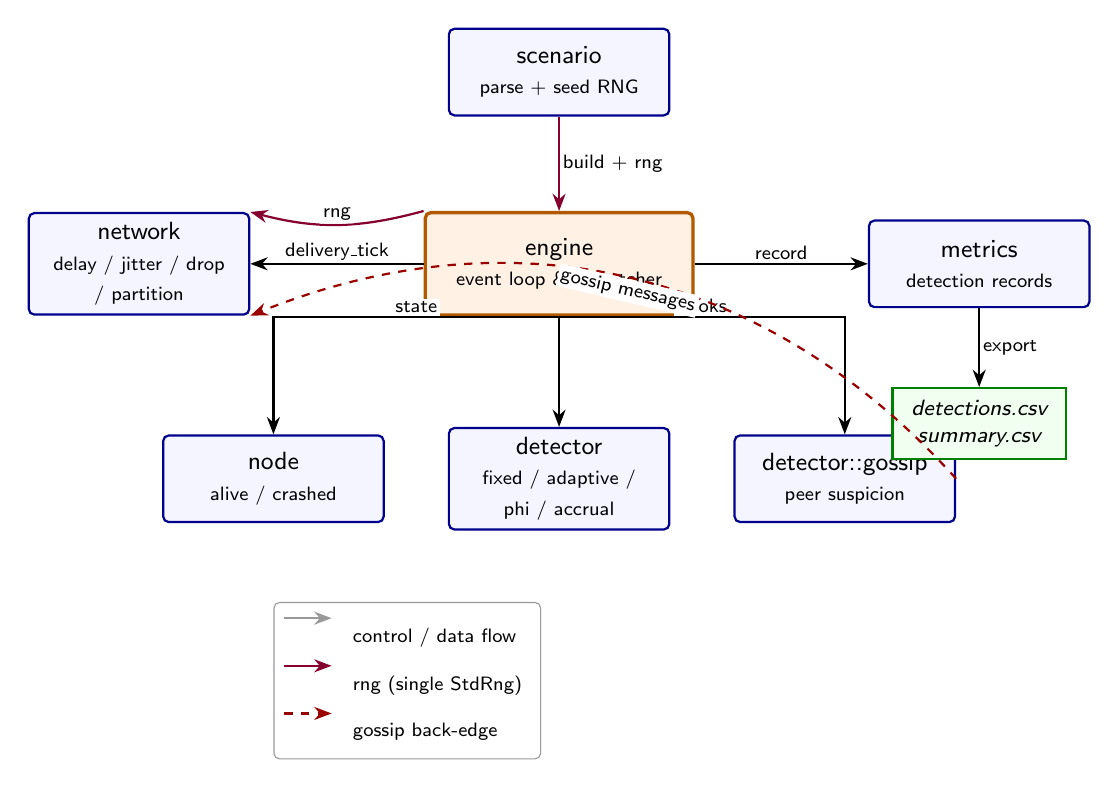
\begin{tikzpicture}[
    font=\sffamily\small,
    node distance=14mm and 18mm,
    every node/.style={align=center},
    %% module box: a service that the Engine calls into
    module/.style={
        draw, rounded corners=2pt, thick,
        minimum width=28mm, minimum height=11mm,
        fill=blue!4, draw=blue!55!black
    },
    %% the central event-loop module
    core/.style={
        draw, rounded corners=2pt, very thick,
        minimum width=34mm, minimum height=13mm,
        fill=orange!10, draw=orange!70!black
    },
    %% terminal artifact (CSV output)
    artifact/.style={
        draw, thick,
        minimum width=22mm, minimum height=9mm,
        fill=green!6, draw=green!50!black,
        font=\sffamily\footnotesize\itshape
    },
    %% data/control flow
    flow/.style={-{Stealth[length=2.2mm]}, thick},
    %% special-case gossip back-edge
    gossip/.style={-{Stealth[length=2.2mm]}, thick, dashed, draw=red!60!black},
    %% rng flow
    rng/.style={-{Stealth[length=2.2mm]}, thick, draw=purple!70!black},
    %% edge label
    elab/.style={font=\sffamily\scriptsize, fill=white, inner sep=1pt}
]

%%-------------------------------------------------------------- nodes
\node[module]                              (scenario)   {scenario\\\scriptsize parse + seed RNG};

\node[core,    below=12mm of scenario]     (engine)     {engine\\\scriptsize event loop \& dispatcher};

\node[module,  left=22mm of engine]        (network)    {network\\\scriptsize delay / jitter / drop\\\scriptsize / partition};

\node[module,  right=22mm of engine]       (metrics)    {metrics\\\scriptsize detection records};

\node[module,  below=14mm of engine]       (detector)   {detector\\\scriptsize fixed / adaptive /\\\scriptsize phi / accrual};

\node[module,  left=8mm of detector]       (node)       {node\\\scriptsize alive / crashed};

\node[module,  right=8mm of detector]      (gossip)     {detector::gossip\\\scriptsize peer suspicion};

\node[artifact, below=10mm of metrics]     (csv)        {detections.csv\\summary.csv};

%%-------------------------------------------------------------- edges
% scenario builds engine; rng enters here
\draw[rng] (scenario) -- node[elab,right] {build + rng} (engine);

% engine queries network for delivery_tick
\draw[flow] (engine.west) -- node[elab,above] {delivery\_tick} (network.east);

% engine writes to metrics
\draw[flow] (engine.east) -- node[elab,above] {record} (metrics.west);

% engine dispatches to nodes (state mutation) and detectors (hooks)
\draw[flow] (engine.south) -| node[elab,pos=0.25,above] {state} (node.north);
\draw[flow] (engine.south) --                                (detector.north);
\draw[flow] (engine.south) -| node[elab,pos=0.25,above] {hooks} (gossip.north);

% rng also flows from engine to network on every delivery_tick call
\draw[rng] (engine.north west) to[bend left=15] node[elab,above,sloped] {rng}  (network.north east);

% gossip is the one detector that produces messages back through the network
\draw[gossip] (gossip.east) to[bend right=35]
    node[elab,sloped,below] {gossip messages}
    (network.south east);

% metrics writes the CSV artifacts
\draw[flow] (metrics) -- node[elab,right] {export} (csv);

%%-------------------------------------------------------------- legend
\matrix [draw=black!40, rounded corners=2pt, fill=white,
         row sep=1pt, column sep=4pt,
         font=\sffamily\scriptsize,
         below=10mm of node, anchor=north west] (legend) {
  \draw[flow]   (0,0) -- (6mm,0); & \node {control / data flow}; \\
  \draw[rng]    (0,0) -- (6mm,0); & \node {rng (single StdRng)};  \\
  \draw[gossip] (0,0) -- (6mm,0); & \node {gossip back-edge};     \\
};

\end{tikzpicture}
\end{document}
                 % just the tikzpicture
%   (wrap it in \begin{figure} ... \end{figure} in the host document)
%
% Required packages (already loaded below for standalone use):
%   tikz, with libraries: positioning, arrows.meta, shapes.geometric, calc

\documentclass[tikz,border=8pt]{standalone}
\usepackage{tikz}
\usetikzlibrary{positioning, arrows.meta, shapes.geometric, calc}

\begin{document}
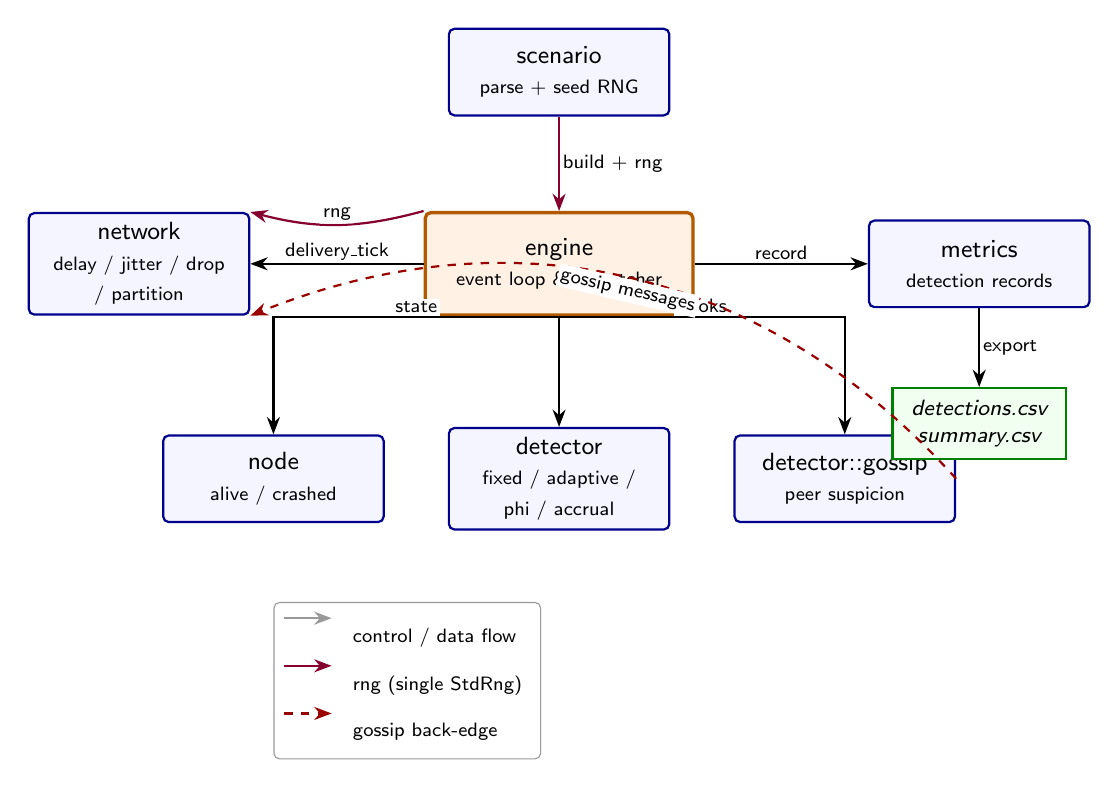
\begin{tikzpicture}[
    font=\sffamily\small,
    node distance=14mm and 18mm,
    every node/.style={align=center},
    %% module box: a service that the Engine calls into
    module/.style={
        draw, rounded corners=2pt, thick,
        minimum width=28mm, minimum height=11mm,
        fill=blue!4, draw=blue!55!black
    },
    %% the central event-loop module
    core/.style={
        draw, rounded corners=2pt, very thick,
        minimum width=34mm, minimum height=13mm,
        fill=orange!10, draw=orange!70!black
    },
    %% terminal artifact (CSV output)
    artifact/.style={
        draw, thick,
        minimum width=22mm, minimum height=9mm,
        fill=green!6, draw=green!50!black,
        font=\sffamily\footnotesize\itshape
    },
    %% data/control flow
    flow/.style={-{Stealth[length=2.2mm]}, thick},
    %% special-case gossip back-edge
    gossip/.style={-{Stealth[length=2.2mm]}, thick, dashed, draw=red!60!black},
    %% rng flow
    rng/.style={-{Stealth[length=2.2mm]}, thick, draw=purple!70!black},
    %% edge label
    elab/.style={font=\sffamily\scriptsize, fill=white, inner sep=1pt}
]

%%-------------------------------------------------------------- nodes
\node[module]                              (scenario)   {scenario\\\scriptsize parse + seed RNG};

\node[core,    below=12mm of scenario]     (engine)     {engine\\\scriptsize event loop \& dispatcher};

\node[module,  left=22mm of engine]        (network)    {network\\\scriptsize delay / jitter / drop\\\scriptsize / partition};

\node[module,  right=22mm of engine]       (metrics)    {metrics\\\scriptsize detection records};

\node[module,  below=14mm of engine]       (detector)   {detector\\\scriptsize fixed / adaptive /\\\scriptsize phi / accrual};

\node[module,  left=8mm of detector]       (node)       {node\\\scriptsize alive / crashed};

\node[module,  right=8mm of detector]      (gossip)     {detector::gossip\\\scriptsize peer suspicion};

\node[artifact, below=10mm of metrics]     (csv)        {detections.csv\\summary.csv};

%%-------------------------------------------------------------- edges
% scenario builds engine; rng enters here
\draw[rng] (scenario) -- node[elab,right] {build + rng} (engine);

% engine queries network for delivery_tick
\draw[flow] (engine.west) -- node[elab,above] {delivery\_tick} (network.east);

% engine writes to metrics
\draw[flow] (engine.east) -- node[elab,above] {record} (metrics.west);

% engine dispatches to nodes (state mutation) and detectors (hooks)
\draw[flow] (engine.south) -| node[elab,pos=0.25,above] {state} (node.north);
\draw[flow] (engine.south) --                                (detector.north);
\draw[flow] (engine.south) -| node[elab,pos=0.25,above] {hooks} (gossip.north);

% rng also flows from engine to network on every delivery_tick call
\draw[rng] (engine.north west) to[bend left=15] node[elab,above,sloped] {rng}  (network.north east);

% gossip is the one detector that produces messages back through the network
\draw[gossip] (gossip.east) to[bend right=35]
    node[elab,sloped,below] {gossip messages}
    (network.south east);

% metrics writes the CSV artifacts
\draw[flow] (metrics) -- node[elab,right] {export} (csv);

%%-------------------------------------------------------------- legend
\matrix [draw=black!40, rounded corners=2pt, fill=white,
         row sep=1pt, column sep=4pt,
         font=\sffamily\scriptsize,
         below=10mm of node, anchor=north west] (legend) {
  \draw[flow]   (0,0) -- (6mm,0); & \node {control / data flow}; \\
  \draw[rng]    (0,0) -- (6mm,0); & \node {rng (single StdRng)};  \\
  \draw[gossip] (0,0) -- (6mm,0); & \node {gossip back-edge};     \\
};

\end{tikzpicture}
\end{document}
